\documentclass[11pt]{article}
\usepackage[margin=0.82in]{geometry}
\usepackage{amsmath,amssymb,amsthm,mathtools}
\usepackage{graphicx}
\usepackage{xcolor}
\usepackage[hidelinks]{hyperref}
\usepackage{microtype}

\newtheorem{theorem}{Theorem}
\newtheorem{corollary}{Corollary}
\newcommand{\A}{\mathcal A}
\newcommand{\F}{\mathbb F}
\newcommand{\C}{\mathbb C}
\newcommand{\otmin}{\otimes_{\min}}
\newcommand{\otmax}{\otimes_{\max}}

\title{Non-WEP coefficients destroy free trigonometric factorization\\
\large A counterexample to the C*-coefficient extension asked in arXiv:2511.06487}
\author{Automated mathematical-discovery candidate (lane 11)}
\date{12 August 2026}

\begin{document}
\maketitle

\noindent\fcolorbox{black}{gray!8}{\parbox{0.94\linewidth}{
\textbf{Status.} Candidate counterexample; current verdict \textbf{likely valid}.
It completely answers the paper's broad question negatively by refuting the
trigonometric theorem for every non-WEP coefficient algebra.  It does not
decide the separate unconstrained self-adjoint-polynomial extension.}}

\section{Source problem}

Jindal, Klep, and McCullough prove in Theorem 1.3 that a
$\mathcal B(\mathcal H)$-valued trigonometric polynomial on the free group
which is positive under every spatial unitary evaluation is a finite sum of
hermitian squares (and, in their infinite-dimensional setting, a single
square) \cite{JKM}.  On PDF page 22, Section 8, they ask whether their results
remain true for arbitrary C*-algebra coefficients:

\begin{center}
 
\includegraphics[width=0.98\linewidth]{figures/open_problem_crop.png}
\end{center}

We keep exactly the source's spatial evaluation convention.  Thus, for a
faithful representation $\pi:\A\to\mathcal B(H)$ and
$p=\sum_{w\in\F_2}a_w w\in\A[\F_2]$, evaluation at a unitary pair
$U=(U_1,U_2)$ on $K$ is
\[
 p(U)=\sum_w \pi(a_w)\otimes U^w\in\mathcal B(H\otimes K).
\]
The result below shows that the answer to the broad question is no.

\section{Proof intuition}

Spatial evaluations see the \emph{minimal} tensor product
$\A\otmin C^*(\F_2)$.  In contrast, an algebraic sum of hermitian squares is
positive in \emph{every} C*-completion, hence in the maximal tensor product.
For an algebra without the weak expectation property (WEP), those two tensor
norms differ.  Choose a finite group-ring tensor $x$ whose maximal norm is
larger than its minimal norm, and place a scalar $\lambda$ strictly between
their squares.  Then
\[
 p=\lambda 1-x^*x
\]
is strictly positive in the minimal completion, so every spatial unitary
evaluation is positive, but it is not positive in the maximal completion.
This rules out not only a single square but every finite sum of squares.

\section{The WEP input}

We use the following theorem of Farenick, Kavruk, and Paulsen
\cite[Theorem 4.3]{FKP}.  For every unital C*-algebra $\A$,
\begin{equation}\label{eq:wep}
 \A\otmin C^*(\F_2)=\A\otmax C^*(\F_2)
 \quad\Longleftrightarrow\quad \A\text{ has WEP}.
\end{equation}
Their statement (take $n=3$) is reproduced below.

\begin{center}
 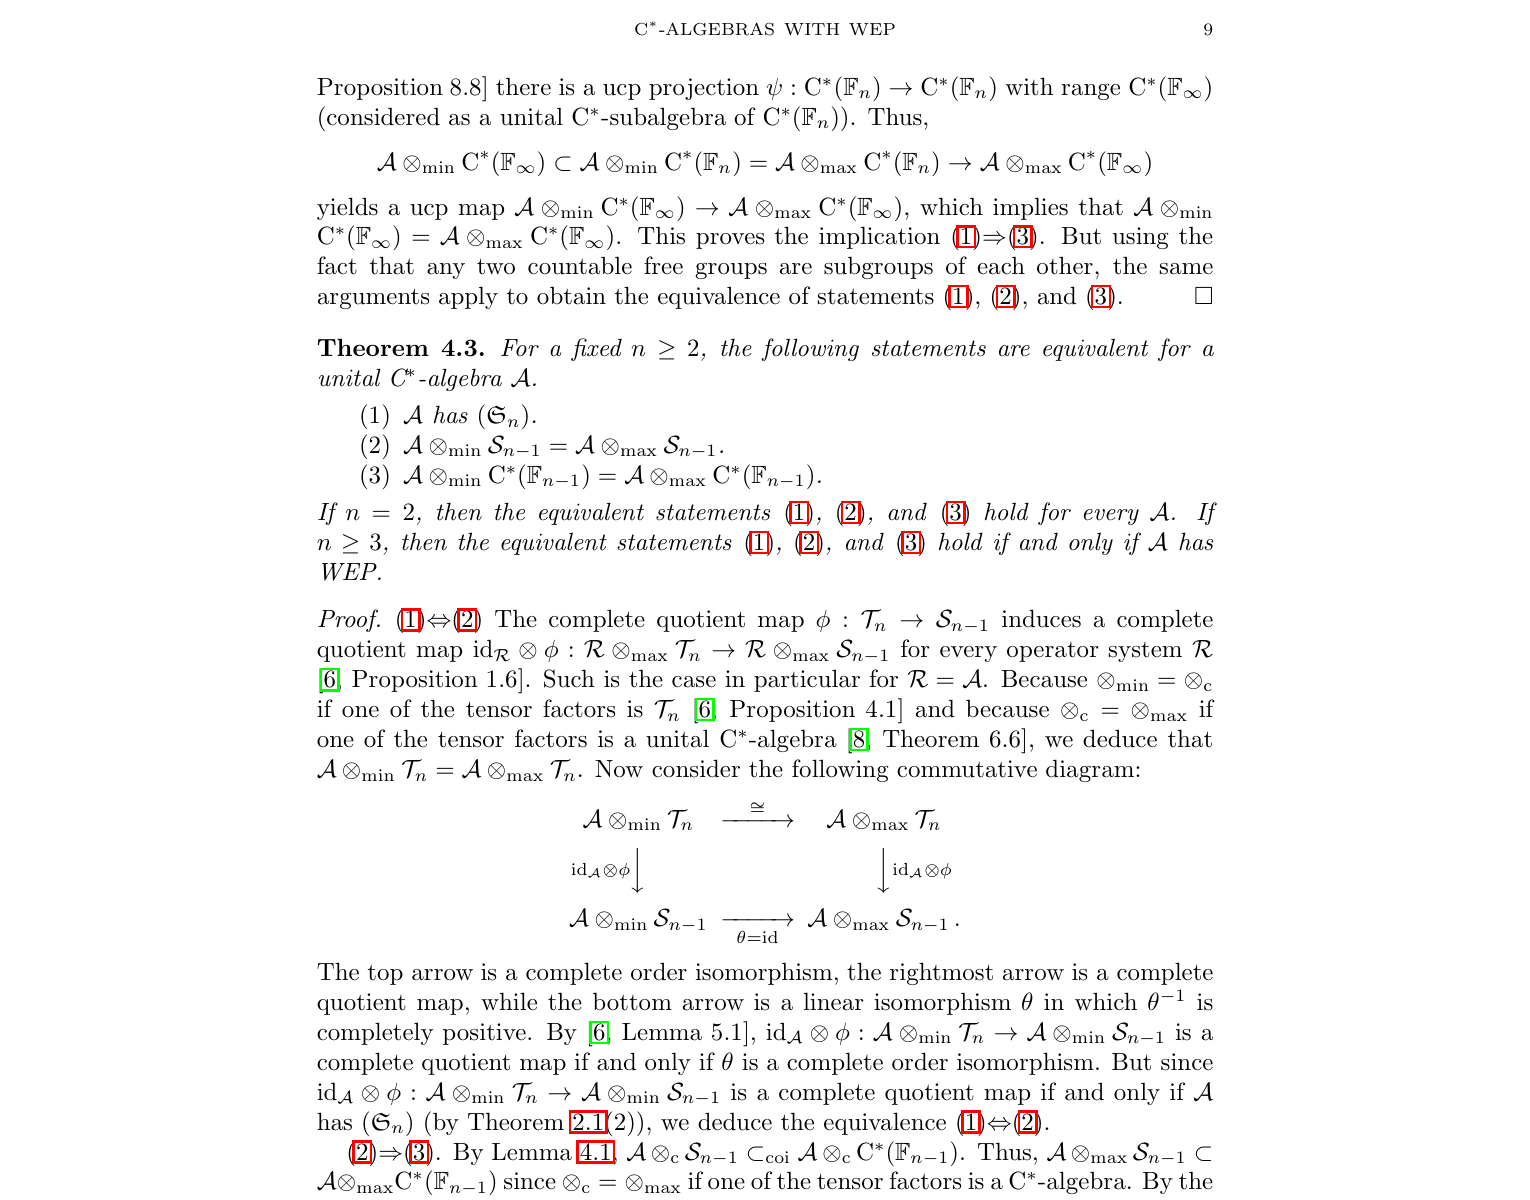
\includegraphics[width=0.92\linewidth]{figures/wep_theorem_crop.png}
\end{center}

The equality in \eqref{eq:wep} means equality of the two C*-norms on the
algebraic tensor product.  Therefore, if $\A$ lacks WEP, some algebraic tensor
has distinct norms.

\section{Counterexample theorem}

\begin{theorem}\label{thm:main}
Let $\A$ be a unital C*-algebra without WEP.  There exist an integer $d$, a
finite element $x\in\A\odot\C[\F_2]$ supported on words of length at most
$d$, and a self-adjoint trigonometric polynomial
\[
 p=\lambda1-x^*x\in\A[\F_2]
\]
of degree at most $2d$ such that:
\begin{enumerate}
 \item $p(U)>0$ for every unitary pair $U$ on every Hilbert space;
 \item $p$ is not a finite sum of hermitian squares in $\A[\F_2]$.
\end{enumerate}
In particular, the C*-coefficient extension of Theorem 1.3 of
\cite{JKM} is false.
\end{theorem}

\begin{proof}
By \eqref{eq:wep}, the minimal and maximal norms on
$\A\odot C^*(\F_2)$ differ.  Hence there is
$y=\sum_{j=1}^m a_j\otimes b_j$ with
$\|y\|_{\max}>\|y\|_{\min}$.  Approximate each $b_j$ in norm by
$c_j\in\C[\F_2]$.  For either tensor norm $\alpha\in\{\min,\max\}$,
\[
 \left\|\sum_j a_j\otimes(b_j-c_j)\right\|_\alpha
 \le \sum_j\|a_j\|\,\|b_j-c_j\|.
\]
Choosing the approximations sufficiently close preserves the strict gap.
Thus, after replacing $y$, we have a finite
$x\in\A\odot\C[\F_2]$ with
\begin{equation}\label{eq:gap}
 \|x\|_{\min}<\|x\|_{\max}.
\end{equation}
Choose a real number
\begin{equation}\label{eq:lambda}
 \|x\|_{\min}^2<\lambda<\|x\|_{\max}^2
\end{equation}
and set $p=\lambda1-x^*x$.

In the minimal tensor product,
\[
 p\ge(\lambda-\|x\|_{\min}^2)1>0.
\]
Every unitary pair $U$ induces a unital *-representation
$\rho_U:C^*(\F_2)\to\mathcal B(K)$.  The spatial evaluation of the source is
the image of $p$ under $\pi\otimes\rho_U$ from the minimal tensor product.
It follows that
\[
 p(U)\ge(\lambda-\|x\|_{\min}^2)I_{H\otimes K}>0.
\]

Suppose, toward a contradiction, that
$p=\sum_{k=1}^N r_k^*r_k$ with $r_k\in\A[\F_2]$.  Under the canonical map
into $\A\otmax C^*(\F_2)$, the right-hand side is positive.  Hence
$\lambda1-x^*x\ge0$ in that C*-algebra.  Positivity would imply
$x^*x\le\lambda1$, and therefore
$\|x\|_{\max}^2\le\lambda$, contradicting \eqref{eq:lambda}.  Thus no finite
sum-of-squares factorization exists.
\end{proof}

\begin{corollary}\label{cor:wep}
If the two-variable trigonometric factorization conclusion of Theorem 1.3 in
\cite{JKM} holds for a unital coefficient algebra $\A$ under spatial
evaluations, then $\A$ has WEP.
\end{corollary}

\begin{proof}
This is the contrapositive of Theorem~\ref{thm:main}.
\end{proof}

Non-WEP algebras exist.  For example, a von Neumann algebra has WEP exactly
when it is injective \cite[Corollary 6.2]{FKP}; thus a standard noninjective
von Neumann algebra such as the free group factor $L(\F_2)$ supplies a
coefficient algebra in Theorem~\ref{thm:main}.  Under the same spatial
evaluation convention, this also shows that the source's preceding blanket
von Neumann-algebra remark needs an injectivity (or a different positivity-
semantics) qualification.

\section{Scope, verification, and novelty}

The construction answers the source's broad question without an explicit
closed formula for $x$: failure of WEP supplies an algebraic norm-gap witness,
and density moves that witness into the finite group ring.  The proof has no
computational dependency.  Verification checked the direction of both tensor
norm inequalities, the preservation of the gap under group-ring
approximation, strict positivity of every spatial evaluation, and the fact
that any finite sum of squares is maximal-positive.

The separate extension of the source's unconstrained self-adjoint-polynomial
Theorem 1.1 is not decided here.  Cayley-transform and symmetry-dilation
attempts produce rational denominators or positivity only on constrained
tuples; no exact implication back from polynomial squares to group-ring
squares was obtained.  Nor is WEP claimed sufficient for exact algebraic
factorization: min=max removes this obstruction, but positivity in a completed
tensor product alone gives no bounded-degree algebraic square certificate.

A bounded search on 12 August 2026 covered the exact title and arXiv id,
\texttt{C*-algebra coefficients}, \texttt{WEP},
\texttt{operator-valued noncommutative trigonometric polynomial}, and their
combinations.  It found the source and general WEP/tensor-product literature,
but no later answer to this concluding problem or this norm-gap
counterexample.  Novelty is plausible, not certified.  Human review should
focus on the intended spatial evaluation convention and the application of
\cite[Theorem 4.3]{FKP} with $n=3$.

\begin{thebibliography}{9}
\bibitem{JKM}
A. Jindal, I. Klep, and S. McCullough,
\emph{Positive operator-valued noncommutative polynomials are squares},
arXiv:2511.06487; Integral Equations Operator Theory 98 (2026), Article 7,
especially Theorem 1.3 and PDF page 22.

\bibitem{FKP}
D. Farenick, A. S. Kavruk, and V. I. Paulsen,
\emph{C*-algebras with the weak expectation property and a multivariable
analogue of Ando's theorem on the numerical radius},
arXiv:1107.0418, especially Theorem 4.3 and Corollary 6.2.
\end{thebibliography}

\end{document}

